\documentclass[a4paper, 11pt]{scrartcl}

\usepackage[utf8]{inputenc} % gestion des accents (source)
\usepackage[T1]{fontenc} % gestion des accents (PDF)
%\usepackage[francais]{babel} % gestion du français
\usepackage[english]{babel} % gestion du français
\usepackage{textcomp} % caractères additionnels
\usepackage{xcolor}
\usepackage{caption}
\usepackage{subcaption}
\usepackage{lmodern} % police de caractères

\newcommand{\jump}{\vspace{0.3cm}}

\usepackage[bookmarks=true]{hyperref} % liens hypertexte
\hypersetup{
  colorlinks,
  citecolor=violet,
  linkcolor=black,
  urlcolor=blue}
%\usepackage{pstricks} % encadrage

\usepackage{graphicx}
\usepackage{caption}
\usepackage{amsmath, amsfonts, amssymb}
%\usepackage{listings}
%\usepackage[fancysections]{polytechnique}
\usepackage{fancyhdr}
\usepackage{eso-pic,xcolor,graphicx}
\definecolor{light-gray}{gray}{0.7}

\pagestyle{fancy}
%\usepackage[top=1in, bottom=1.25in, left=1in, right=1in]{geometry}

%\lhead{Convex Neural Networks} 
%\chead{\today}
%\rhead{Eloïse \textsc{Berthier}}

\title{On Convex Neural Networks}
\author{Eloïse Berthier}
\date{\today}
\subtitle{Mathematical Foundations of Data Science}


\begin{document}

\setcounter{secnumdepth}{3}
\setlength{\parindent}{0cm}

\maketitle
%\fontfamily{lmss}\selectfont

\everymath{\displaystyle}

\abstract{
\emph{1/2 page: What problem(s) is studied ? 
Why is it relevant ? 
What solution(s) is proposed ? 
Which contributions (theory, numerics, etc) ? 
}}

\newpage

\section{Introduction}

While the use of neural networks has dramatically increased the performance of some recognition systems, there still lacks a clear mathematical understanding of this success. One of the key issues is that optimizing neural networks is a non-convex problem, hence training algorithms may not return a global minimum.

Yet in practice, training large neural networks often results in satisfying solutions, which are empirically considered \textit{not too far} from a global minimum. Thus it suggests that there may be some implicit assumptions on the data or on the model that are usually verified and could explain this regularity, somehow making the problem \textit{more convex} than at first sight.\\

There have been several attempts to study this phenomenon, heading in different directions.

Some rely on convex relaxations of the original optimization problem. \cite{zhang2016convexified} defines a convex relaxation for training convolutional neural networks. They show that in the case of a two-layer CNN, the generalization error of the solution to the convex relaxed problem converges to that of the best possible two-layer CNN.

In \cite{haeffele2017global} are studied conditions under which the optimization landscape for the non-convex optimization problem is such that all critical points are either global minimizers or saddle points.

There is also a series of some very recent contributions on the problem: \cite{du2018agradient}, \cite{du2018bgradient} and \cite{zou2018stochastic}. They rely on the analysis of the dynamics of the prediction space rather than of the parameter space, the former being governed by the spectral property of a Gram matrix. If the data is \textit{not degenerate}, this Gram matrix’s least eigenvalue is lower bounded, and randomly initialized gradient descent linearly converges to a global optimum.\\

In this report, we concentrate on another approach called \textit{convex neural networks}. The core idea was introduced by \cite{bengio2006convex} and focuses on one hidden-layer neural networks. Instead of optimizing the weights of a network with a fixed number of hidden units, we could consider the equivalent problem of optimizing on the set of all the possible hidden unit functions. The training problem is convex with respect to the parameters of the model (which are now only the ouput weights).

Of course, while this approach solves the non-convexity issue, it introduces some other difficulties. These are extensively studied in \cite{bach2017breaking}, on which we will mainly focus in this report. A complete analysis of the generalization performance of convex neural networks is derived, in particular showing that high-dimensional non-linear variable selection may be achieved, without any strong assumption regarding the data. Yet this approach requires to solve a convex problem in infinite dimension and is only possible if the non-convex subproblem of adding a new hidden unit can be solved efficiently. Finding a polynomial-time algorithm solving this subproblem induced by the conditional gradient method is still an open question.

\cite{chizat2018global} focuses on solving the same convex problem, but avoids the potentially NP-hard problem of optimizing with conditional gradient. Instead, they discretize the unknown measure as a mixture of particles. This approach is inspired by optimal transport and brings strong asymptotical global optimality garantees for gradient flow optimization. It also provides simple numerical experiments.\\

Looking at all these different approaches, we may notice some recurrent patterns in the assumptions that are commonly made:

\begin{itemize}
\item \textit{one hidden-layer models}: most of the articles focus on simple neural network models, that already include a wide variety of classical supervised learning configurations, but do not directly cover deep neural networks.
\item \textit{over parametrization}: all the good generalization properties are derived in the case of an over parametrizing model, yet the key question is \textit{how much} over parametrization is needed.
\item \textit{positive homogeneity}: most of the results are achieved in the case of positively homogeneous activation functions. It could explain the experimental advantage of using ReLU functions over others in deep learning.
\item \textit{proper initialization}: several articles rely on the conservation of an initial regularity through the optimizing process, for instance using gradient flows, and so emphasize the role of the initialization.
\end{itemize}



\section{Defining a Convex Problem}

non convex problem

the convex problem

number of hidden units

sample complexity

\section{Theoretical Analysis}

\subsection{Errors decomposition}
3 errors decomposition.
Speak about the last two

\subsection{Approxmiation error ?}


\subsection{Generalization error}


\section{An Optimization Problem}

\subsection{Frank Wolfe}

\subsection{NP hard}


\section{The Particle Gradient Flow Approach}

A more general result, can be applied to this problem

\section{Numerical Experiments}

Main body (~10 pages) : 
Presentation of the method(s). 
Theoretical guarantees. 
Numerics. 

\section{Conclusion and perspectives}

Conclusion and perspective (~1 page)
Summary of the result obtained: pros and cons (limitation, problems, error in the articles, etc)
Possible improvement/extension

\bibliographystyle{apalike}
\bibliography{biblio.bib}

 
\begin{figure}[h]
\centering
\begin{subfigure}{.5\textwidth}
  \centering
  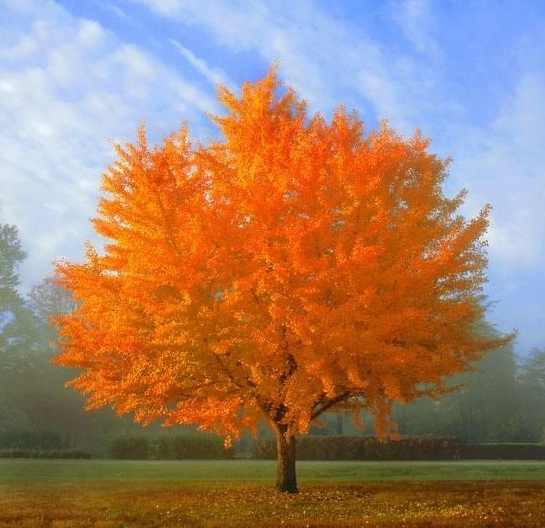
\includegraphics[width=\linewidth]{tree.jpg}
  \caption{Average return during the gradient ascent}
  \label{fig:sub3}
\end{subfigure}%
\begin{subfigure}{.5\textwidth}
  \centering
  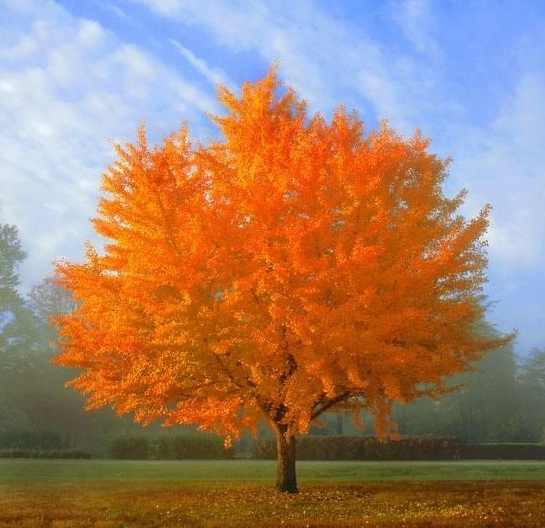
\includegraphics[width=\linewidth]{tree.jpg}
  \caption{Mean parameter during the gradient ascent}
  \label{fig:sub4}
\end{subfigure}%
\end{figure}



\end{document}
